% §5 Setup (compressed from Violation Landscape)

\label{sec:violation_landscape}

We evaluate OntoCoDec in two deployment configurations: greedy S1 (DR\,$\leq$\,0.21\%, $+$10\% latency) and beam S1 (near-zero violations, 1.39$\times$ latency); zero-shot evaluation (\S\ref{sec:scierc-results}; Appendix~\ref{app:cross-model-zs}) serves as a diagnostic probe for the fine-tuned setting (relation F1 (R-F1) 40--46\%).

\paragraph{Setup.}
We evaluate on SciERC~\cite{luan2018scierc} (551 test sentences, 7 relations, $\bar{\kappa}{=}0.333$) and DocRED~\cite{yao2019docred} (998 development documents; test annotations are not publicly available; 96 relations, $\bar{\kappa}{=}0.842$).
RE type constraints are extracted from observed type pairs in training data (neither dataset provides a standalone ontology specification); EE constraints on WikiEvents (\S\ref{sec:wikievents}) derive from the KAIROS ontology.
All constraints are schema-level, independent of evaluation splits.
Primary model: Qwen3-8B~\cite{qwen2025qwen3}, zero-shot greedy decoding; cross-model validation in Appendix~\ref{app:cross-model-zs}, composability with fine-tuning in \S\ref{sec:composability}.
LoRA hyperparameters (rank, $\alpha$, learning rate) were tuned on SciERC and transferred to DocRED without dataset-specific optimization; given the substantial schema complexity difference (7 vs.\ 96 relations), this transfer may underestimate DocRED fine-tuning potential.
Our R-F1 range (40--46\% under LoRA) is consistent with recent LLM-based generative RE evaluations on these benchmarks, where document-level closed IE without gold entity spans typically achieves 35--50\%~\cite{wadhwa2023revisiting}; supervised span-based methods operating under different assumptions (gold entity spans, dedicated architectures) are not directly comparable.
For reference, the supervised end-to-end SOTA on SciERC achieves 41.6\% strict Rel-F1 (PL-Marker~\cite{ye2022packed}) and 36.8\% (PURE~\cite{zhong2021frustratingly}); while evaluation protocols differ, our 40--46\% R-F1 range under LoRA falls within a comparable band.
DocRED development documents were used for evaluation only.
Prompt templates and reproducibility details (hyperparameters, dataset statistics) in Appendices~\ref{app:prompts} and~\ref{app:reproducibility}.
Four violation categories: \textbf{DR} (type pair $\notin \sigma(r)$), \textbf{RV} (relation $\notin \mathcal{R}$), \textbf{ET} (entity type $\notin \mathcal{E}$), \textbf{CF} (conflicting types across triples).
Baseline DR: 15.37\% (SciERC), 18.46\% (DocRED); schema-informed prompting reduces DR by 62\% but is per-relation unreliable (Appendix~\ref{app:per-relation-landscape}).

% Figure 6: Violation composition (placed before figure* to land on page 6)
\begin{figure}[t]
\centering
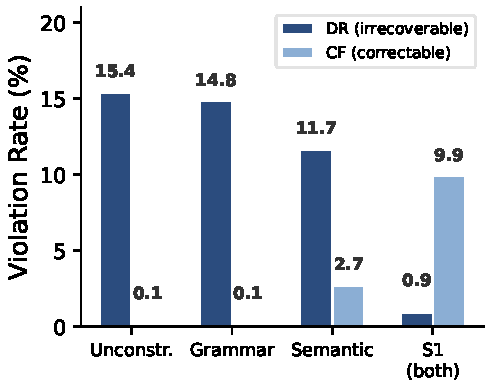
\includegraphics[width=\columnwidth]{figures/fig_violation_composition.pdf}
\caption{Violation composition across constraint configurations (SciERC, Qwen3-8B, zero-shot). As layers compose, DR (irrecoverable) drops 94\% while CF (correctable) becomes the sole residual, a severity downgrade from ontology-invalid to cross-triple type inconsistency.}
\label{fig:violation-composition}
\end{figure}

% Figures 4+5 side-by-side (spanning both columns)
\begin{figure*}[t]
\centering
\begin{minipage}[t]{0.48\textwidth}
  \centering
  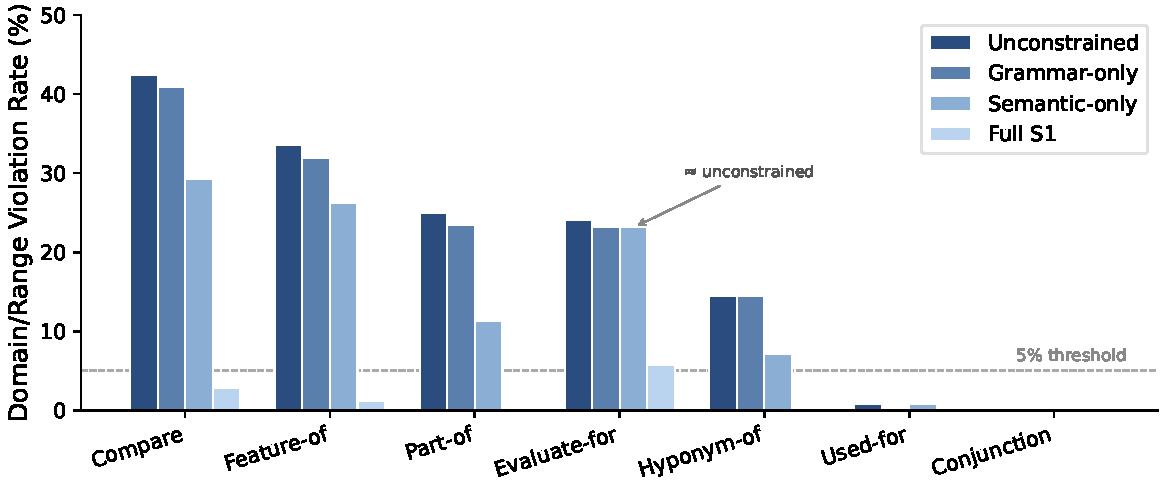
\includegraphics[width=\linewidth]{figures/fig2_per_relation_dr.pdf}
  \caption{Per-relation DR violation rates on SciERC (Qwen3-8B, unconstrained). Rates correlate with constraint tightness $\kappa(r)$. Llama-3.1-8B shows similar patterns (Appendix~\ref{app:llama-per-relation}).}
  \label{fig:per_relation_dr}
\end{minipage}%
\hfill
\begin{minipage}[t]{0.48\textwidth}
  \centering
  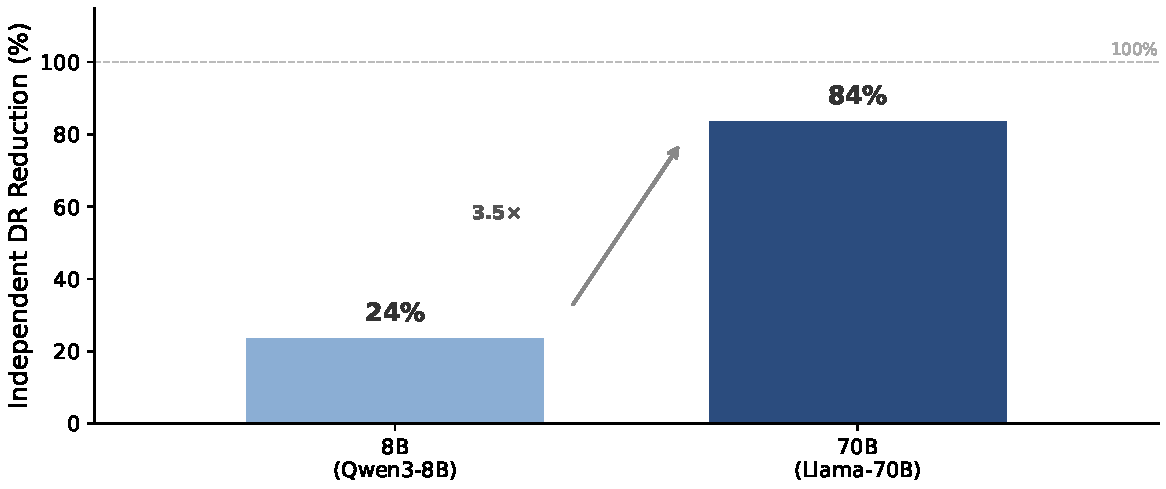
\includegraphics[width=\linewidth]{figures/fig_scale_dependency.pdf}
  \caption{Scale-dependent layer interaction: the semantic layer's independent DR reduction grows from 24\% at 8B to 84\% at 70B, reducing reliance on grammar-enforced vocabulary.}
  \label{fig:scale-dependency}
\end{minipage}
\end{figure*}
